\title{17. Objemy a povrchy těles, řezy těles rovinou}

\author{Jan Peroutka}
\maketitle

\section{Objemy a povrchy těles, řezy těles rovinou}

\subsection{Obecně k tělesům}
Tělesa jsou trojrozměrné geometrické útvary, jejichž objem a povrch se dá vyjádřit pomocí matematických vzorců. Dále je lze zobrazit a analyzovat pomocí řezů rovinou.

\subsection{Hranol}
\begin{itemize}
    \item Objem: $V = S_p \cdot v$, kde $S_p$ je obsah podstavy a $v$ výška.
    \item Povrch: $S = 2 \cdot S_p + S_{pl}$, kde $S_{pl}$ je obsah pláště (součet obsahů stěn mezi podstavami).
\end{itemize}
\textbf{Řezy hranolem:} mohou být rovnoběžné s podstavou (vypadá jako podstava), nebo kolmé na podstavu (obdélníky nebo pravoúhlé tvary).

\subsection{Válec}
\begin{itemize}
    \item Objem: $V = \pi r^2 v$
    \item Povrch: $S = 2\pi r^2 + 2\pi r v$
\end{itemize}
\textbf{Řezy válcem:}
\begin{itemize}
    \item Řez rovinou rovnoběžnou s osou: obdélník
    \item Řez kolmý na osu: kruh
\end{itemize}

\subsection{Kužel}
\begin{itemize}
    \item Objem: $V = \frac{1}{3} \pi r^2 v$
    \item Povrch: $S = \pi r^2 + \pi r s$, kde $s$ je délka strany (tvořící).
\end{itemize}
\textbf{Řezy kuželem:}
\begin{itemize}
    \item Kolmý řez osou: rovnoramenný trojúhelník
    \item Rovnoběžný s podstavou: kruh menšího poloměru
\end{itemize}

\subsection{Koule}
\begin{itemize}
    \item Objem: $V = \frac{4}{3} \pi r^3$
    \item Povrch: $S = 4\pi r^2$
\end{itemize}
\textbf{Řezy koulí:} libovolný rovinný řez koulí je kruh. Největší řez (středový) je kruh s poloměrem $r$.

\subsection{Poznámka k řezům}
Řezy těles nám pomáhají pochopit jejich vnitřní strukturu. Často se využívají např. v technických výkresech, deskriptivní geometrii nebo fyzice.

\subsubsection*{Konstrukční pravidla pro rýsování řezu hranolem}

\begin{enumerate}
    \item \textbf{Dva body leží na stejné stěně} $\Rightarrow$ \emph{spojujeme je přímou úsečkou.}  
    Pokud zadané body leží na téže stěně tělesa, můžeme je přímo spojit úsečkou. Tato úsečka pak tvoří část řezu.

    \item \textbf{Tři body, z nichž dva leží na jedné stěně a třetí na protější} $\Rightarrow$ \emph{určíme směr a vedeme rovnoběžku.}  
    Například body $A$ a $B$ leží na přední stěně, bod $C$ na zadní: spojíme $A$ a $B$, čímž určíme směr, a tímto směrem vedeme rovnoběžku přes bod $C$.

    \item \textbf{Dva body leží ve dvou různých stěnách, třetí leží ve třetí stěně} $\Rightarrow$ \emph{určíme průsečík pomocí roviny.}  
    Pokud body $L,J$ a $K$ leží ve dvou různých stěnách (např. přední a boční), určíme rovinu jejich spojením. Tato rovina protne třetí stěnu (např. pravou) – najdeme průsečík této roviny s hranou dané stěny (např. $BF$) a tím získáme další bod (např. $M$). Pokud třetí bod (např. $K$) už leží v této rovině, lze ho rovnou použít a spojit s ostatními.

    \begin{figure}
        \centering
        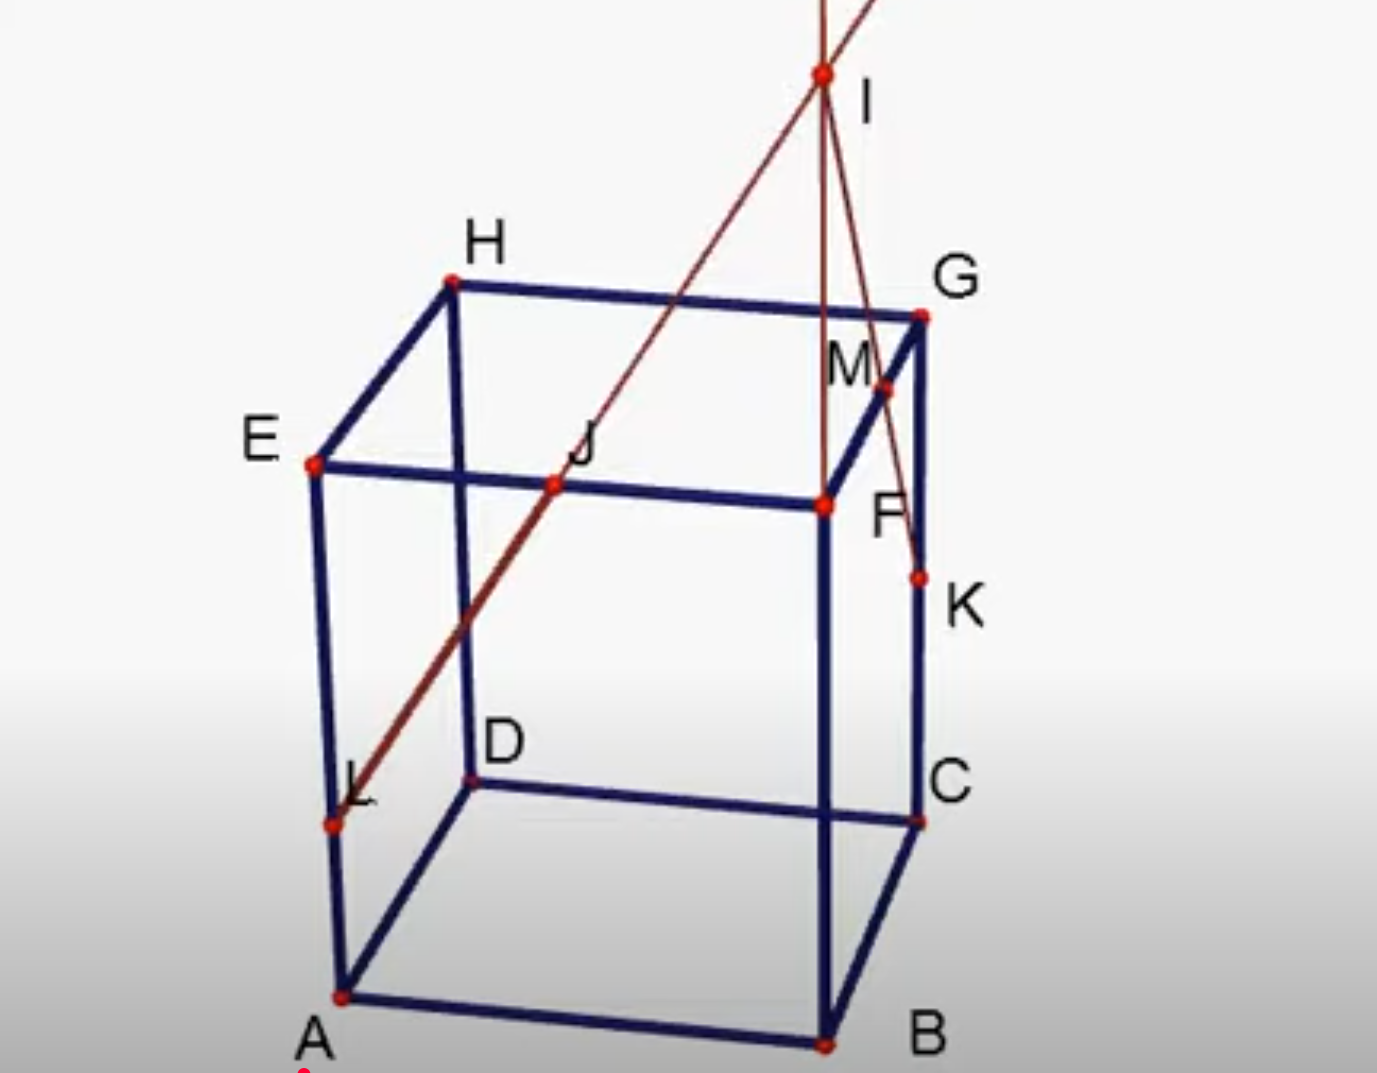
\includegraphics[width=0.5\linewidth]{img/16_objemy_rez.png}
        \caption{3. pravidlo v akci}
    \end{figure}

    \item \textbf{Řezová čára je vždy spojitá a tvořená úsečkami.}  
    Musí ležet v jednotlivých stěnách tělesa a nesmí se „lámat“ uvnitř jedné stěny.

    \item \textbf{Řez vždy začíná a končí na hraně tělesa.}  
    Žádná část řezu nesmí ležet mimo stěnu nebo končit „ve vzduchu“.

    \item \textbf{Rovina řezu nemůže částečně ležet v hraně – buď celá, nebo vůbec.}  
    Pokud rovina řezu prochází hranou, musí celá ležet v rovině této stěny.
\end{enumerate}
